\documentclass{extbook}[14pt]
\usepackage{multicol, enumerate, enumitem, hyperref, color, soul, setspace, parskip, fancyhdr, amssymb, amsthm, amsmath, latexsym, units, mathtools}
\everymath{\displaystyle}
\usepackage[headsep=0.5cm,headheight=0cm, left=1 in,right= 1 in,top= 1 in,bottom= 1 in]{geometry}
\usepackage{dashrule}  % Package to use the command below to create lines between items
\newcommand{\litem}[1]{\item #1

\rule{\textwidth}{0.4pt}}
\pagestyle{fancy}
\lhead{}
\chead{Answer Key for Module6 Version C}
\rhead{}
\lfoot{7334-5530}
\cfoot{}
\rfoot{test}
\begin{document}
\textbf{This key should allow you to understand why you choose the option you did (beyond just getting a question right or wrong). \href{https://xronos.clas.ufl.edu/mac1105spring2020/courseDescriptionAndMisc/Exams/LearningFromResults}{More instructions on how to use this key can be found here}.}

\textbf{If you have a suggestion to make the keys better, \href{https://forms.gle/CZkbZmPbC9XALEE88}{please fill out the short survey here}.}

\textit{Note: This key is auto-generated and may contain issues and/or errors. The keys are reviewed after each exam to ensure grading is done accurately. If there are issues (like duplicate options), they are noted in the offline gradebook. The keys are a work-in-progress to give students as many resources to improve as possible.}

\rule{\textwidth}{0.4pt}

\begin{enumerate}\litem{
Describe the zero behavior of the zero $x = -9$ of the polynomial below.
\[ f(x) = -2(x - 4)^{9}(x + 4)^{7}(x + 9)^{3}(x - 9)^{2} \]The solution is the graph below.
    \begin{center}
        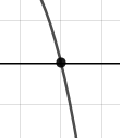
\includegraphics[width=0.3\textwidth]{../Figures/polyZeroBehaviorAC.png}
    \end{center}

\textbf{General Comment:} You will need to sketch the entire graph, then zoom in on the zero the question asks about.
}
\litem{
Write an equation that \textit{could} represent the graph below.

\begin{center}
    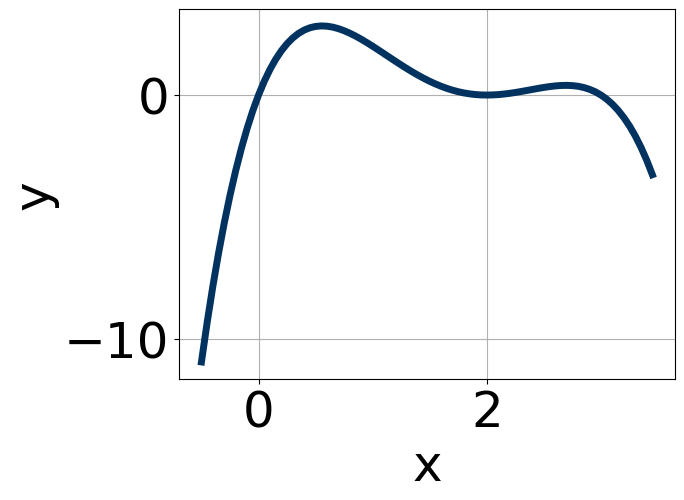
\includegraphics[width=0.5\textwidth]{../Figures/polyGraphToFunctionC.png}
\end{center}


The solution is \( 3(x + 4)^{7} (x + 3)^{5} (x + 1)^{5} \).\begin{enumerate}[label=\Alph*.]
\textbf{Plausible alternative answers include:}The factor $(x + 4)$ should have an odd power and the leading coefficient should be the opposite sign.
The factors $-4$ and $-3$ have have been odd power.
* This is the correct option.
The factor $-4$ should have been an odd power.
This corresponds to the leading coefficient being the opposite value than it should be.
\end{enumerate}

\textbf{General Comment:} General Comments: Draw the x-axis to determine which zeros are touching (and so have even multiplicity) or cross (and have odd multiplicity).
}
\litem{
Construct the lowest-degree polynomial given the zeros below.
\[ 1, \frac{7}{4}, \text{ and } \frac{5}{3} \]The solution is \( 12x^{3} -53 x^{2} +76 x -35 \).\begin{enumerate}[label=\Alph*.]
\textbf{Plausible alternative answers include:}$12x^{3} +53 x^{2} +76 x + 35$, which corresponds to multiplying out $(x + 1)(4x + 7)(3x + 5)$.
$12x^{3} +13 x^{2} -34 x -35$, which corresponds to multiplying out $(x + 1)(4x + 7)(3x -5)$.
* $12x^{3} -53 x^{2} +76 x -35$, which is the correct option.
$12x^{3} -53 x^{2} +76 x + 35$, which corresponds to multiplying everything correctly except the constant term.
$12x^{3} -29 x^{2} -6 x + 35$, which corresponds to multiplying out $(x + 1)(4x -7)(3x -5)$.
\end{enumerate}

\textbf{General Comment:} To construct the lowest-degree polynomial, you want to multiply out $(x -1)(4x -7)(3x -5)$
}
\litem{
Describe the zero behavior of the zero $x = 9$ of the polynomial below.
\[ f(x) = 2(x - 7)^{6}(x + 7)^{4}(x + 9)^{8}(x - 9)^{7} \]The solution is the graph below.
    \begin{center}
        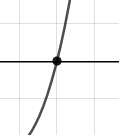
\includegraphics[width=0.3\textwidth]{../Figures/polyZeroBehaviorCopyDC.png}
    \end{center}

\textbf{General Comment:} You will need to sketch the entire graph, then zoom in on the zero the question asks about.
}
\litem{
Construct the lowest-degree polynomial given the zeros below.
\[ 7, \frac{-7}{3}, \text{ and } 4 \]The solution is \( 3x^{3} -26 x^{2} +7 x + 196 \).\begin{enumerate}[label=\Alph*.]
\textbf{Plausible alternative answers include:}$3x^{3} +26 x^{2} +7 x -196$, which corresponds to multiplying out $(x + 7)(3x -7)(x + 4)$.
$3x^{3} -26 x^{2} +7 x -196$, which corresponds to multiplying everything correctly except the constant term.
$3x^{3} +16 x^{2} -63 x -196$, which corresponds to multiplying out $(x + 7)(3x + 7)(x -4)$.
$3x^{3} +2 x^{2} -105 x + 196$, which corresponds to multiplying out $(x + 7)(3x -7)(x -4)$.
* $3x^{3} -26 x^{2} +7 x + 196$, which is the correct option.
\end{enumerate}

\textbf{General Comment:} To construct the lowest-degree polynomial, you want to multiply out $(x -7)(3x + 7)(x -4)$
}
\litem{
Describe the end behavior of the polynomial below.
\[ f(x) = 7(x + 6)^{3}(x - 6)^{6}(x - 3)^{3}(x + 3)^{3} \]The solution is the graph below.
    \begin{center}
        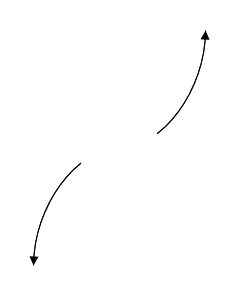
\includegraphics[width=0.3\textwidth]{../Figures/polyEndBehaviorCopyDC.png}
    \end{center}

\textbf{General Comment:} Remember that end behavior is determined by the leading coefficient AND whether the \textbf{sum} of the multiplicities is positive or negative.
}
\litem{
Construct the lowest-degree polynomial given the zeros below.
\[ 2 - 2 i \text{ and } 2 \]The solution is \( x^{3} -6 x^{2} +16 x -16 \).\begin{enumerate}[label=\Alph*.]
\textbf{Plausible alternative answers include:}$x^{3} + x^{2} -4 x + 4$, which corresponds to multiplying out $(x -2)(x -2)$.
$x^{3} +6 x^{2} +16 x + 16$, which corresponds to multiplying out $(x-(2 - 2 i))(x-(2 + 2 i))(x + 2)$.
$x^{3} + x^{2} +0 x -4$, which corresponds to multiplying out $(x + 2)(x -2)$.
* $x^{3} -6 x^{2} +16 x -16$, which is the correct option.
This corresponds to making an unanticipated error or not understanding how to use nonreal complex numbers to create the lowest-degree polynomial. If you chose this and are not sure what you did wrong, please contact the coordinator for help.
\end{enumerate}

\textbf{General Comment:} Remember that the conjugate of $a+bi$ is $a-bi$. Since these zeros always come in pairs, we need to multiply out $(x-(2 - 2 i))(x-(2 + 2 i))(x-(2))$.
}
\litem{
Write an equation that \textit{could} represent the graph below.

\begin{center}
    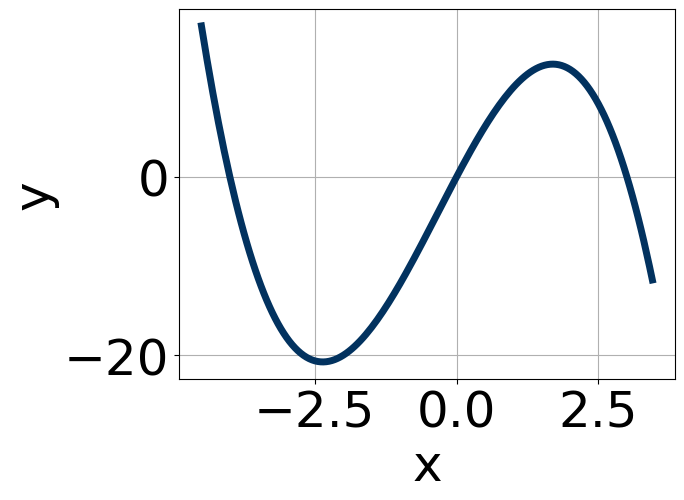
\includegraphics[width=0.5\textwidth]{../Figures/polyGraphToFunctionCopyC.png}
\end{center}


The solution is \( -2x^{8} (x + 2)^{7} (x + 4)^{9} \).\begin{enumerate}[label=\Alph*.]
\textbf{Plausible alternative answers include:}This corresponds to the leading coefficient being the opposite value than it should be.
The factor $0$ should have an even power and the factor $-2$ should have an odd power.
* This is the correct option.
The factor $(x + 2)$ should have an odd power.
The factor $(x + 4)$ should have an odd power and the leading coefficient should be the opposite sign.
\end{enumerate}

\textbf{General Comment:} General Comments: Draw the x-axis to determine which zeros are touching (and so have even multiplicity) or cross (and have odd multiplicity).
}
\litem{
Construct the lowest-degree polynomial given the zeros below.
\[ -2 - 4 i \text{ and } 3 \]The solution is \( x^{3} + x^{2} +8 x -60 \).\begin{enumerate}[label=\Alph*.]
\textbf{Plausible alternative answers include:}* $x^{3} + x^{2} +8 x -60$, which is the correct option.
$x^{3} + x^{2} -x -6$, which corresponds to multiplying out $(x + 2)(x -3)$.
$x^{3} + x^{2} +x -12$, which corresponds to multiplying out $(x + 4)(x -3)$.
$x^{3} -1 x^{2} +8 x + 60$, which corresponds to multiplying out $(x-(-2 - 4 i))(x-(-2 + 4 i))(x + 3)$.
This corresponds to making an unanticipated error or not understanding how to use nonreal complex numbers to create the lowest-degree polynomial. If you chose this and are not sure what you did wrong, please contact the coordinator for help.
\end{enumerate}

\textbf{General Comment:} Remember that the conjugate of $a+bi$ is $a-bi$. Since these zeros always come in pairs, we need to multiply out $(x-(-2 - 4 i))(x-(-2 + 4 i))(x-(3))$.
}
\litem{
Describe the end behavior of the polynomial below.
\[ f(x) = 7(x + 5)^{4}(x - 5)^{5}(x + 9)^{2}(x - 9)^{3} \]The solution is the graph below.
    \begin{center}
        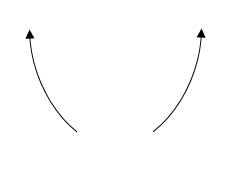
\includegraphics[width=0.3\textwidth]{../Figures/polyEndBehaviorCC.png}
    \end{center}

\textbf{General Comment:} Remember that end behavior is determined by the leading coefficient AND whether the \textbf{sum} of the multiplicities is positive or negative.
}
\end{enumerate}

\end{document}